\documentclass[authoryear]{tex/labreport}

% python terminal: 
% import os, shutil;new='jakob_daniel_18409686_MEEN30020_2020-21_assign1_report.pdf';os.replace(r'main.pdf',new); newPath = shutil.copy(new, '../')


% latexmk -lualatex -auxdir=".aux" -shell-escape -recorder-  main.tex
% lualatex  -shell-escape -aux-directory=".aux"  "main.tex"
% makeindex main.nlo -s nomencl.ist -o main.nls
% biber  "main.bcf"


\AtEndPreamble{
\hypersetup{    
pdfkeywords={Mechanics of Solids, Bending, Torsion, Circular Cross-sections},
}
}

\firstname{Daniel}
\familyname{Jakob}
\modulecode{MEEN30020}
\modulename{Mechanics of Solids II}
\stage{3}
\major{School of Mechanical \& Materials Engineering}
\institution{UCD}
\studentnumber{18409686}
\reporttitle{Lab Report}
\subtitle{Combined Bending \& Torsion}
\modulecoord{Dr. Neal Murphy}
\labta{Mr. Daniel Dreelan}

\DTMsavedate{submitdate}{2021-04-22}
\DTMsavedate{duedate}{2021-04-23}
\DTMsavedate{labdate}{2021-04-05}
\date{\DTMusedate{submitdate}}

\tikzset{
  >=stealth', % Change default arrow tip
}

\usemintedstyle{daniel}

\usepackage{nicefrac}

\usetikzlibrary{external}
\tikzexternalize[prefix=tikzexternalize/,optimize command away=\includepdf]
\makeatletter
    \tikzset{%
        external/system call={%
            lualatex %
                \tikzexternalcheckshellescape %
                -halt-on-error %
                -interaction=batchmode %
                -output-directory=".aux" %
                -jobname "\image" %
                "\texsource"%
        },
        /pgf/images/include external/.code={%
            \includegraphics{.aux/#1}%
        },%
    }
\makeatother

\usepackage{bm}
%\usepackage{xcolor}
\definecolor{mynumber}{rgb}{0.4, 0.4, 0.4}
\definecolor{mytext}{rgb}{0, 0, 0}

\newcommand{\matr}[1]{\boldsymbol{\mathbf{#1}}}

%%%%%%%%%%%%%%%%%%%%%%%%%%%%%%%%%%%%%%%%%%%%%%%%%%%%%%%%%%%%%%%%%%%%%%%%%%%%%%%%%%%%%%%%%
%	TITLE PAGE
%%%%%%%%%%%%%%%%%%%%%%%%%%%%%%%%%%%%%%%%%%%%%%%%%%%%%%%%%%%%%%%%%%%%%%%%%%%%%%%%%%%%%%%%%
\begin{document}
\newcolumntype{Z}{S[round-mode=places, round-precision=3,table-number-alignment = center] }
\pdfbookmark[1]{Title Page}{title page}
\maketitle % Insert the title, author and date
\thispagestyle{empty} % No header, footer or page number on title page 

\begin{figure}[H] % UCD Crest picture
\begin{center}

\includegraphics[width=0.15\textwidth]{ucd_crest}
\end{center}
\end{figure}
\makeatletter
\begin{center}
\begin{tabular}{r l}
\\
Module Coordinator: & \@modulecoord\\ % Instructor/supervisor
Date Due: & \DTMusedate{duedate} \\  % Date the report is due
Lab T.A.: & \@labta \\
Date of Lab: & \DTMusedate{labdate}
\\\\
\end{tabular}
\end{center}
\makeatother

\pdfbookmark[1]{Abstract}{abstract}
\begin{abstract}
\noindent\normalsize In this experiment, a force is applied to copper specimen attached to a loading plate where bending, torsion, and any combination of the two can be applied. The resulting deflections and remaining deflections are measured for corresponding proportions of bending and torsion. The results are compared to two theories regarding bending and torsion in materials, max shear stress yield criterion and maximum principal stress failure criterion. Ultimately, the former reflects the material's behaviour better. 
\end{abstract}

\clearpage
\thispagestyle{empty} % No header, footer or page number on title page 
\pdfbookmark[1]{\contentsname}{toc}
\tableofcontents
\clearpage
\thispagestyle{assessmentform}

\begin{figure}[H] % UCD Crest picture
\begin{center}
\vspace{-3em}

\includegraphics[width=0.1\textwidth,left]{ucd_crest}
\end{center}
\end{figure}
\vspace{-2.5em}
\section*{Assessment Submission Form}
\addcontentsline{toc}{section}{Assessment Submission Form}
\renewcommand{\arraystretch}{1.5}
\makeatletter

\begin{table}[htpb]
\begin{tabularx}{\textwidth}{|l|X|}
\hline
Student Name       & \@firstname\;\@familyname \\ \hline
Student Number     & \@studentnumber \\ \hline
Assessment Title   & \@subtitle \\ \hline
Module Code        & \@modulecode \\ \hline
Module Title       & \@modulename \\ \hline
Module Coordinator & \@modulecoord \\ \hline
Date Submitted     & \DTMusedate{submitdate} \\ \hline
Date Received      &  \\ \hline
Grade/Mark         &  \\ \hline
\end{tabularx}
\end{table}
\makeatother
\renewcommand{\arraystretch}{1.1}
\textbf{A SIGNED COPY OF THIS FORM MUST ACCOMPANY ALL SUBMISSIONS FOR ASSESSMENT.\\\\STUDENTS SHOULD KEEP A COPY OF ALL WORK SUBMITTED.\\\\Procedures for Submission and Late Submission\\}
Ensure that you have checked the Adult Education Centre's procedures for the submission of assessments.\\
\textbf{Note:} There are penalties for the late submission of assessments. For further information please see the Adult Education \textit{Assessment Guidelines} publication or the website at \href{http://www.ucd.ie/adulted}{www.ucd.ie/adulted}.\\\\
\textbf{Plagiarism} is the unacknowledged inclusion of another person's writings or ideas or works, in any formally presented work (including essays, examinations, projects, laboratory reports or presentations). The penalties associated with plagiarism are designed to impose sanctions that reflect the seriousness of the University's commitment to academic integrity. Ensure that you have read the University's \textit{\textbf{Briefing for Students on Academic Integrity and Plagiarism}} and the UCD \textit{\textbf{Plagiarism Statement, Plagiarism Policy and Procedures}}, (\href{http://www.ucd.ie/registrar/}{http://www.ucd.ie/registrar/}).\\\\
\noindent\fbox{%
    \parbox{0.9825\textwidth}{%
        \textbf{Declaration of Authorship}\\ I declare that all material in this assessment is my own work except where there is clear acknowledgement and appropriate reference to the work of others.\\\\
        \begin{tabular}{lm{5cm}ll}
        \textbf{Signed} & 
\includegraphics[height=1.5cm,keepaspectratio]{signature} & \textbf{Date} & \DTMusedate{submitdate}
        \end{tabular}
    }%
}
\newpage

\pagestyle{myheadings} % Change page style to one with header and page numbers
%\addcontentsline{toc}{chapter}{Nomenclature}

% \subsection*{Symbols}

\nomenclature[S]{\(F\)}{Force [N]}
\nomenclature[S]{\(W\)}{Load [N]}
\nomenclature[S]{\(\delta\)}{Deflection [mm]}
\nomenclature[S]{\(\sigma\)}{stress [MPa]}
\nomenclature[S]{\(\varepsilon\)}{deformation [mm]}
\nomenclature[S]{\(M\)}{Moment [Nm]}
\nomenclature[S]{\(\mathcal{F}\)}{Form factor [$-$]}
\nomenclature[S]{\(I\)}{Second moment of area $\left[\si{\meter\tothe{4}}\right]$}

\nomenclature[A]{\(c\)}{\href{https://physics.nist.gov/cgi-bin/cuu/Value?c}
{Speed of light in a vacuum}
\nomunit{\SI{299792458}{\meter\per\second}}}
\nomenclature[A]{\(h\)}{\href{https://physics.nist.gov/cgi-bin/cuu/Value?h}
{Planck constant}
\nomunit{\SI{6.62607015e-34}{\joule\per\hertz}}}
\nomenclature[A]{\(G\)}{\href{https://physics.nist.gov/cgi-bin/cuu/Value?bg}
{Gravitational constant} 
\nomunit{\SI{6.67430e-11}{\meter\cubed\per\kilogram\per\second\squared}}}

% % \subsection*{Abbreviations}
% \nomenclature[A]{LHS}{Left-hand side}
% \nomenclature[A]{RHS}{Right-hand side}
% \nomenclature[A]{dir}{Direction}
% \nomenclature[A]{NA}{Neutral axis}

% \subsection*{Sub- and Superscripts}
\nomenclature[U]{y}{Yield}
\nomenclature[U]{p}{Plastic}

\printnomenclature


%*******************************************************
% Acronyms
%*******************************************************
%\phantomsection
%\pdfbookmark[1]{Acronyms}{acronyms}
%\markboth{\spacedlowsmallcaps{Acronyms}}{\spacedlowsmallcaps{Acronyms}}
%\chapter*{Acronyms}
\textbf{Acronyms, Abbreviations and Initialisms}
\begin{acronym}[UMLX]
    \acro{DRY}{Don't Repeat Yourself}
    \acro{API}{Application Programming Interface}
    \acro{UML}{Unified Modeling Language}
\end{acronym}


\clearpage
%%%%%%%%%%%%%%%%%%%%%%%%%%%%%%%%%%%%%%%%%%%%%%%%%%%%%%%%%%%%%%%%%%%%%%%%%%%%%%%%%%%%%%%%%
%	INTRODUCTION
%%%%%%%%%%%%%%%%%%%%%%%%%%%%%%%%%%%%%%%%%%%%%%%%%%%%%%%%%%%%%%%%%%%%%%%%%%%%%%%%%%%%%%%%%
\section{Introduction}
\label{sec:intro}
% Why Did You Do What You Did? An explanation of the background to the experiment.
% Provide some background on the area. Why are fluid machines important? What are they used for?
% Cite relevant literature such as textbooks and academic journals to support your discussion.

Bending and torsion are important natural phenomena which must be understood thoroughly by engineers when designing structures (buildings, bridges, etc.). Bending and torsion depend on many factors including material, geometry and nature of force being applied. Lots of theory has been developed over the last couple of centuries attempting to describe these mathematically; however, theory is useless if it does not apply to real life. This lab experiment seeks out to determine the relationship between bending and torsion. A little copper specimen is being examined in a specialised test rig produced by GUNT GmbH where forces can be applied to the specimen in pure bending, pure torsion and all combinations in between. The portion of force acting in torsion and the portion acting in bending is determined by the angle at which angle the force is placed at on the loading plate (see: \cref{subsec:equip}). According to the \textit{max shear stress yield criterion}, the \textit{effective} stress of the specimen is independent of the angle at which the force is applied,  however according the the \textit{maximum principal stress failure criterion} the stress \textit{is} dependent on the angle.
\begin{longlisting}
    \caption{\texttt{makelink.m} function m-file}
    \inputminted[bgcolor=lightgray!30,escapeinside=££]{matlab}{code/makelink.m}
    \label{lst:makelink}
\end{longlisting}
%---------------------------------------------------------------------------------------%
%	OBJECTIVES
%---------------------------------------------------------------------------------------%

\subsection{Objectives}
\label{subsec:objectives}
% Scope and objectives of the experimental investigation.
% Writing Style Passive style. Past tense is generally accepted as the most appropriate grammatical style for technical reports. For example, version (i) here is very much preferred:(i) "The apparatus was calibrated prior to the experiment", (ii) "We calibrated the apparatus before we conducted the experiment" (please avoid this style). Further  guidance on report writing is available in Holman [1]. Students are referred to Strunk and White [2]for guidance on writing style.
The objective of this experiment is to examine 2 copper specimens in the test rig by inserting one specimen and iteratively applying more load at a certain angle --- which dictates whether the specimen is placed under bending or torsion --- until the material experiences non-elastic deformation (i.e., has exceeded its elastic limit) and then unloading the weights and then measuring what the change in length of the specimen is, its remaining deformation, $\Delta w$. This is repeated for the other angles desired to be examined and then the test is run in reverse angle order for a second specimen. Once all of the data has been collected, the forces and remaining deformations are used to determine whether or not the angle played a role on the deflection of the specimen. \ac{DRY}
%---------------------------------------------------------------------------------------%
%	THEORY
%---------------------------------------------------------------------------------------%
\subsection{Theory}
\label{subsec:theory}
% Using the lab handout and and the literature you've already cited describe the theoretical background for the fluid machine under investigation.
% Work through the various equations needed to describe the performance of the fluid machine and explain what they mean.
%What does Theory have to Say? Where appropriate, include a brief description of the theoretical basis of the work.
The max shear stress yield \ac{DRY} criterion says:
\begin{equation}
    \tau_\text{max} = \frac{F}{2A}
\end{equation}
\begin{conditions}
    \tau & shear stress \\
    F & force applied \\
    A & area\\
    \frac{F}{A} &  $\sigma_\text{axial}$  
\end{conditions}
at the yield point, $\sigma_\text{axial}$ equals $\sigma_\text{yield}$ and in 3D state of stress $\tau_\text{max, 3D} = \nicefrac{\sigma_\text{yield}}{2}$, therefore:  $2\tau_\text{max, 3D}=\sigma_\text{yield}$, this is also called the effective stress. In this test the effective stress $\sigma_\text{eff}$ equals $\nicefrac{4FR}{\pi r^3}$ which is independent from $\phi$ meaning the angle at which the force was applied at on the loading plate does not affect the stress on the specimen \ac{API}. 

For brittle materials, the maximum principal stress failure criterion says:
\begin{equation}
    \sigma_1 = \frac{2FR}{\pi r^3}(1+\cos\phi) 
\end{equation}
which means the angle does affect the stress in the specimen. 
As discussed in \cref{subsec:equip}, pure \ac{API} bending takes place at $\phi = \SI{0}{\degree}\Rightarrow\cos\phi=1$, meaning there is yielding at $F_\text{bend}=\left(\nicefrac{\pi r^3}{4R}\right)\sigma_\text{yield}$, conversely, pure torsion  takes place at $\phi = \SI{90}{\degree}\Rightarrow\cos\phi=0$ meaning yielding at $F_\text{tor}=\left(\nicefrac{\pi r^3}{2R}\right)\sigma_\text{yield}=2F_\text{bend}$. 
%%%%%%%%%%%%%%%%%%%%%%%%%%%%%%%%%%%%%%%%%%%%%%%%%%%%%%%%%%%%%%%%%%%%%%%%%%%%%%%%%%%%%%%%%
%	EXPERIMENTAL METHODS
%%%%%%%%%%%%%%%%%%%%%%%%%%%%%%%%%%%%%%%%%%%%%%%%%%%%%%%%%%%%%%%%%%%%%%%%%%%%%%%%%%%%%%%%%
\section{Methodology}
\label{sec:methods}
\subsection{Equipment and Instrumentation}
\label{subsec:equip}
% Describe the measurement facility. Take photographs of the facility and label them and/or create a drawing of the system.
% Brief description of the equipment and instrumentation and of the techniques used in the lab.
The lab equipment consisted of the test rig, the weights and specimens. There are four weights, \SI{1}{\newton}, \SI{2}{\newton}, \SI{4}{\newton} and \SI{8}{\newton}. 2 identical copper specimens will be used during the course of the experiment, see \cref{fig:specimen}. The specimen is a hollow, dumbbell-shaped cylinder. It is fitted to the rig via a clamping mechanism. 
\begin{figure}[htb]
    \centering
    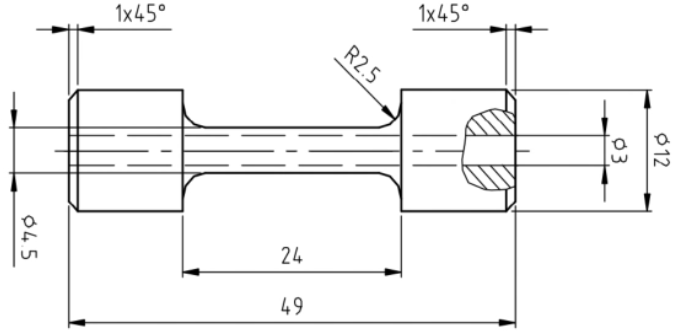
\includegraphics[width=0.75\linewidth]{specimen.png}
    \caption{Specimen geometry and dimensions \cite{gunt:2009}}
    \label{fig:specimen}
\end{figure}
The test rig has several elements: the hook from which the load weights are hung, the counterweights, the measuring gauge, the cable pulley system and the magnetic foot which keeps in place the measuring gauge as seen in \cref{fig:rig}. The counterweight is present in the rig to mitigate the effects of a shear force, $V$, being applied to the specimen. A shear force would just obfuscate results and be generally a nuisance. The gauge is in units of \SI[parse-numbers=false]{\nicefrac{10}{100}}{\milli\meter} which equals \SI{E-5}{\meter}. 
\tikzsetnextfilename{rig}
\begin{figure}[htb]
    \centering
    \begin{tikzpicture}[every text node part/.style={align=center}]
        % Include the image in a node
        
        \node [
            above right,
            inner sep=0] (image) at (0,0) {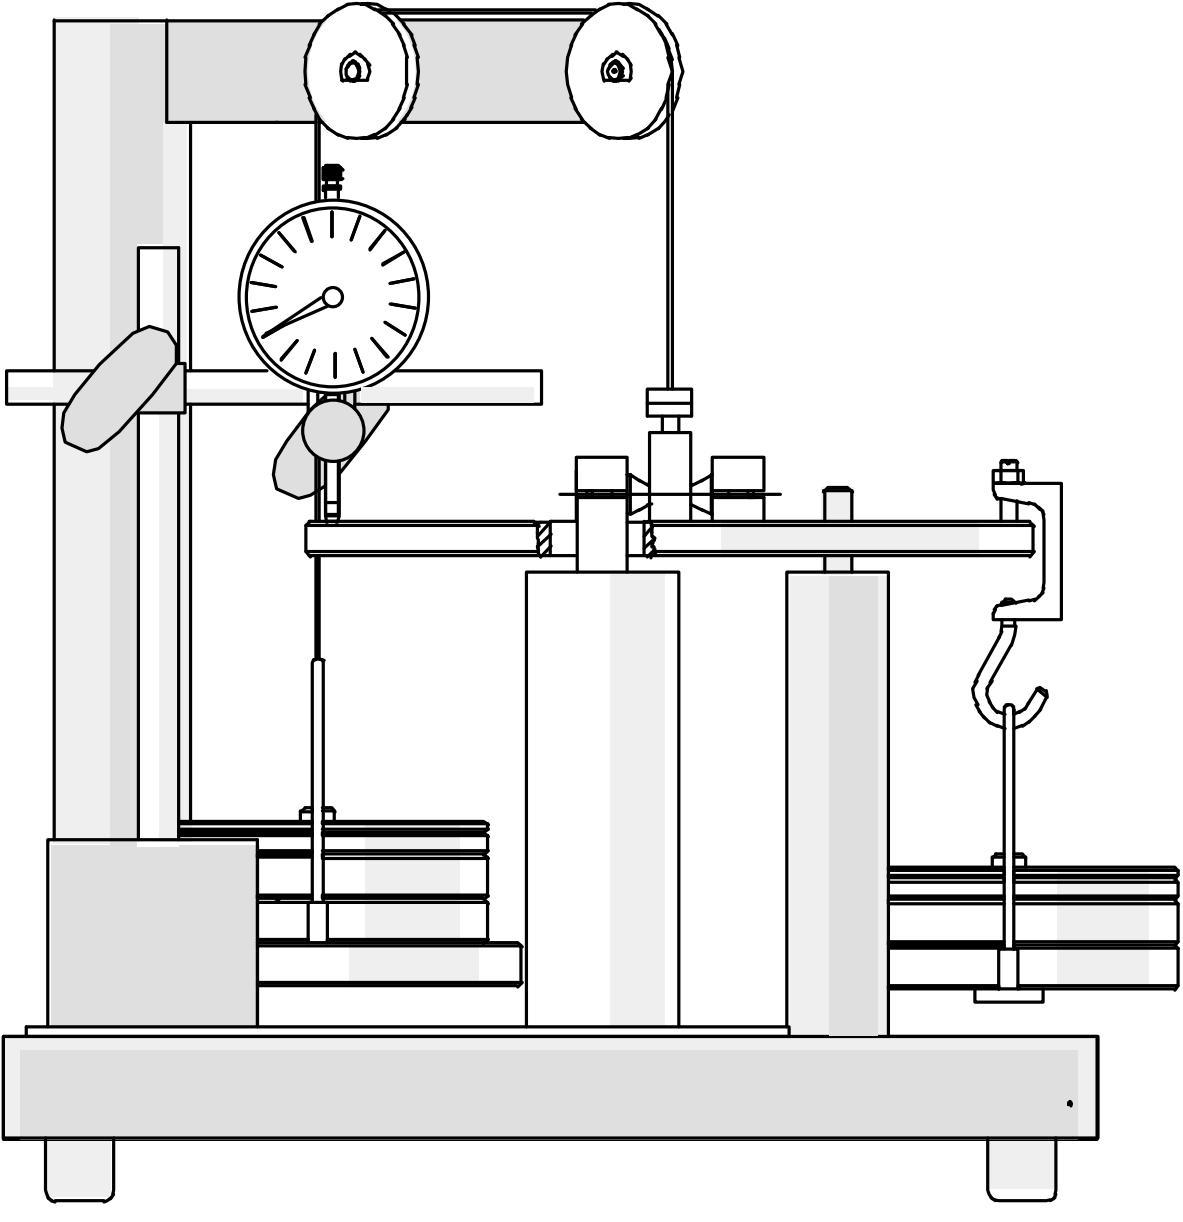
\includegraphics[width=0.5\textwidth]{guntrig}};
        
        % Create scope with normalized axes
        \begin{scope}[
        x={($0.1*(image.south east)$)},
        y={($0.1*(image.north west)$)}]
        
        %Grid
            %\draw[lightgray,step=0.5] (image.south west) grid (image.north east);
        
        %Axes' labels
            %\foreach \x in {0,1,...,10} { \node [below] at (\x,0) {\x}; }
            %\foreach \y in {0,1,...,10} { \node [left] at (0,\y) {\y};}
        
        % Labels
            \draw[latex-, very thick,green] (2.8,7.5) -- ++(-3,0)
            node[left,black]{\small Measuring\\gauge};
            
            \draw[stealth-, very thick,green] (5.5,9.5) -- ++(1,0)
            node[right,black]{\small Cable with reversing\\pulley for counterweight};
    
            \draw[stealth-, very thick,green] (3.5,2.75) -- ++(-3.75,1)
            node[left,black]{\small Counterweight};
    
            \draw[stealth-, very thick,green] (1.5,2) -- ++(-2,0)
            node[left,black]{\small Magnetic foot\\for measuring};
    
            \draw[stealth-, very thick,green] (7,3.75) -- ++(1.8,0)
            node[right,black]{\small Supporting column};
    
            \draw[stealth-, very thick,green] (7.75,5.5) -- ++(0,1)
            node[above,black]{\small Loading Plate};
    
            \draw[stealth-, very thick,green] (9,2.5) -- ++(1.25,0)
            node[right,black]{\small Load Weight};
    
            \draw[stealth-, very thick,green] (8.5,1) -- ++(1.5,0)
            node[right,black]{\small Frame};
        
        \end{scope}
        
\end{tikzpicture}
    \caption{Rig Diagram \cite{gunt:2009}}
    \label{fig:rig}
\end{figure}
\cref{fig:loadingplate} displays a plan view of the loading plate of the test rig. The specimen is attached to the loading plate and the base of the rig by the 2 clamping bridges. The quarter circle in the bottom left of the image is where the angle of force is chosen. There are little divots for where a pin which carries the force can be placed. In the configuration shown in the figure, the angle $\phi$ is \SI{0}{\degree} which corresponds to \href{run:./file.txt}{File.txt} pure bending in the specimen which can be intuitively seen by inspection of the how the specimen is orientated in relation to the force. If the force-pin were place at the divot which is shown at the bottom of the quarter-circle, $\phi$ would be \SI{90}{\degree} and pure torsion would take place in the specimen, the cylinder would be twisted. 
\begin{figure}[htb]
    \centering
    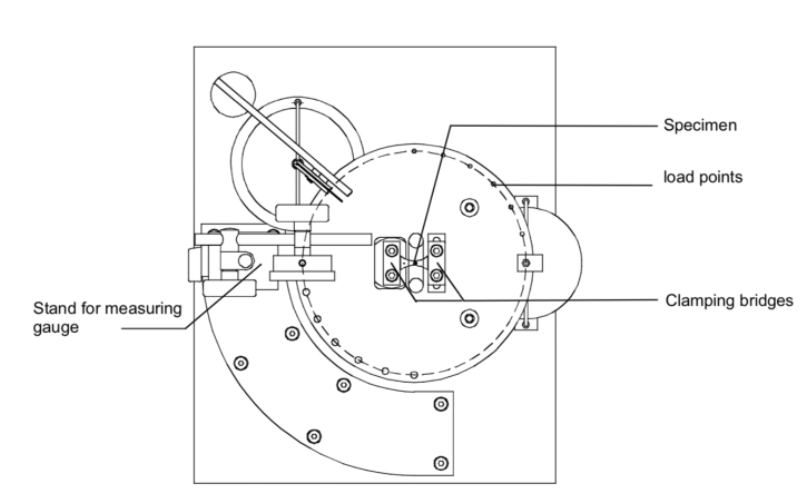
\includegraphics[width=0.75\linewidth]{planview.png}
    \caption{Plan view of loading plate \cite{gunt:2009}}
    \label{fig:loadingplate}
\end{figure}
\subsection{Experimental Procedure}
\label{subsec:procedure}
% List the experimental procedure and note any key observations that should be taken into account (how long should you wait for the flow to stabilise before taking a reading etc).
% Describe the experimental procedure in such a way that somebody else could reproduce the work and obtain the same results. Do not include your results in this section, just explain how the experiment was carried out.
First, one side of the first specimen is inserted into the clamping mechanism connected to the loading plate and secured with an Allen key. The loading plate is lowered and the other half of the specimen is clamped ot the base machine. A close check is made to make sure the two planes of the clamp facing each other are indeed parallel. The test is started at position $\phi=\SI{0}{\degree}$, meaning pure bending, by rotating the loading plate to align the force-pin in the according divot. A load is applied to the specimen by adding weights to the counterweight, starting at \SI{8}{\newton}. The deflection, $w$ and remaining deflection, $\Delta w$ are measured for the load applied. Then weight is added in \SI{1}{\newton} increments, and again the deflections are measured. This is repeated until $\Delta w$ reads 10 units of \SI[parse-numbers=false]{\nicefrac{1}{100}}{\milli\meter}. Then, the weights are taken off, the plate is rotated so the pin is placed in the divot corresponding to \SI{45}{\degree}, this produces a combination of bending and torsion in the specimen and the measuring gauge is zeroed. The \SI{8}{\newton} weight is applied again and the process above is repeated, and is finished by rotating the plate to \SI{90}{\degree} and repeating once more. Then, the specimen is removed and a new specimen is inserted, and the method is repeated, however, this time process is started at \SI{90}{\degree} rather than \SI{0}{\degree} as before and is done in reverse, ending at \SI{0}{\degree}. This results in six sets of data, the load, $F$, deflection and remaining deflection for the three angles for the 2 runs. 

Once all the data has been collected, some preliminary work must be done wherein a form of normalisation must be carried out, specifically, a load value for a remaining deflection value of \SI[parse-numbers=false]{\nicefrac{10}{100}}{\milli\meter} must be obtained for all loading positions and runs. This can be achieved in many ways, but in this experiment, a linear interpolation was conducted in the form of plotting a line chart for the load and the remaining deflection. This needed only to be done in one of the sets of data, by inspection of \cref{tbl:results}, under run 2, $\phi=\SI{0}{\degree}$, it can be seen that remaining deflection skips from \SI{9E-5}{\meter} to \SI{12E-5}{\meter}, meaning a value of force for \SI{10E-5}{\meter} is not obtained. \cref{fig:interp} graphically displays the interpolation carried out: a value of $\approx$\SI{15.4}{\newton} is obtained. 
%%%%%%%%%%%%%%%%%%%%%%%%%%%%%%%%%%%%%%%%%%%%%%%%%%%%%%%%%%%%%%%%%%%%%%%%%%%%%%%%%%%%%%%%%
%	EXPERIMENTAL RESULTS
%%%%%%%%%%%%%%%%%%%%%%%%%%%%%%%%%%%%%%%%%%%%%%%%%%%%%%%%%%%%%%%%%%%%%%%%%%%%%%%%%%%%%%%%%
\section{Experimental Results}
\label{sec:results}
%Using the equations described above plot your measure\-ments on neat graphs and present the results.
\setlength\tabcolsep{5pt}
\begin{table}[htb]
    \small
    \centering
    \caption{Table of Results}
    \label{tbl:results}
    \begin{tabular}{rcccccc}
    \toprule
    \multicolumn{7}{c}{\textbf{Run 1}}\\ \cmidrule{2-7}
    \multicolumn{1}{c}{} & \multicolumn{2}{c}{0\si{\degree}} & \multicolumn{2}{c}{45\si{\degree}}  & \multicolumn{2}{c}{90\si{\degree}} \\ \cmidrule(lr){2-3} \cmidrule(lr){4-5} \cmidrule(lr){6-7}
    \multicolumn{1}{c}{\begin{tabular}[c]{@{}c@{}}Load \\ {[}N{]}\end{tabular}} & \multicolumn{1}{c}{\begin{tabular}[c]{@{}c@{}}Deflection \\ {$\sbk{\SI{E-5}{\meter}}$}\end{tabular}} & \multicolumn{1}{c}{\begin{tabular}[c]{@{}c@{}}Remaining \\ Deflection \\ {$\sbk{\SI{E-5}{\meter}}$}\end{tabular}} & \multicolumn{1}{c}{\begin{tabular}[c]{@{}c@{}}Deflection \\ {$\sbk{\SI{E-5}{\meter}}$}\end{tabular}} & \multicolumn{1}{c}{\begin{tabular}[c]{@{}c@{}}Remaining \\ Deflection \\ {$\sbk{\SI{E-5}{\meter}}$}\end{tabular}} & \multicolumn{1}{c}{\begin{tabular}[c]{@{}c@{}}Deflection \\ {$\sbk{\SI{E-5}{\meter}}$}\end{tabular}} & \multicolumn{1}{c}{\begin{tabular}[c]{@{}c@{}}Remaining \\ Deflection \\ {$\sbk{\SI{E-5}{\meter}}$}\end{tabular}} \\ \midrule
    8                                & 97                          & 0                                                              & 111                                                                                                   & 0                                                                                         & 126                                                                                                      & 1                                                                                                                                                                                               \\
    9                                & 111                         & 0                                                              & 126                                                                                                   & 2                                                                                         & 142                                                                                                      & 2                                                                                                                                                                                               \\
    10                               & 122                         & 0                                                              & 141                                                                                                   & 3                                                                                         & 158                                                                                                      & 3                                                                                                                                                                                              \\
    11                               & 135                         & 2                                                              & 155                                                                                                   & 4                                                                                         & 175                                                                                                      & 4                                                                                                                                                                                               \\
    12                               & 147                         & 2                                                              & 169                                                                                                   & 5                                                                                         & 194                                                                                                      & 6                                                                                                                                                  \\
    13                               & 160                         & 5                                                              & 185                                                                                                   & 6                                                                                         & 211                                                                                                      & 8                                                                                                                                                                                             \\
    14                               & 176                         & 8                                                              & 202                                                                                                   & 7                                                                                         & 230                                                                                                      & 10                                                                                                                                                                                              \\
    15                               & 195                         & 10                                                             & 219                                                                                                   & 10                                                                                        & $-$                                                                                                      & $-$                                                                                                                                                                                           \\
    \multicolumn{7}{c}{\textbf{Run 2}}                                                                                                                                                                                                                                                                                                                                                                                                                                                                                                                                                                                                        \\ \cmidrule{2-7}
    \multicolumn{1}{l}{}             & \multicolumn{2}{c}{90\si{\degree}}                                                                                                                                                                            & \multicolumn{2}{c}{45\si{\degree}}                                                                                                                                                                           & \multicolumn{2}{c}{0\si{\degree}}                                                                                                                                                                           \\ \cmidrule(lr){2-3} \cmidrule(lr){4-5} \cmidrule(lr){6-7}
    \multicolumn{1}{c}{\begin{tabular}[c]{@{}c@{}}Load \\ {[}N{]}\end{tabular}} & \multicolumn{1}{c}{\begin{tabular}[c]{@{}c@{}}Deflection \\ {$\sbk{\SI{E-5}{\meter}}$}\end{tabular}} & \multicolumn{1}{c}{\begin{tabular}[c]{@{}c@{}}Remaining \\ Deflection \\ {$\sbk{\SI{E-5}{\meter}}$}\end{tabular}} & \multicolumn{1}{c}{\begin{tabular}[c]{@{}c@{}}Deflection \\ {$\sbk{\SI{E-5}{\meter}}$}\end{tabular}} & \multicolumn{1}{c}{\begin{tabular}[c]{@{}c@{}}Remaining \\ Deflection \\ {$\sbk{\SI{E-5}{\meter}}$}\end{tabular}} & \multicolumn{1}{c}{\begin{tabular}[c]{@{}c@{}}Deflection \\ {$\sbk{\SI{E-5}{\meter}}$}\end{tabular}} & \multicolumn{1}{c}{\begin{tabular}[c]{@{}c@{}}Remaining \\ Deflection \\ {$\sbk{\SI{E-5}{\meter}}$}\end{tabular}} \\ \midrule
    8                                & 121                                                                                         & 2                                                                                                                                                                                                 & 108                                                                                                      & 1                                                                                          & 93    & 0                                                                                                  \\
    9                                & 138                                                                                         & 3                                                                                                                                                                                                 & 121                                                                                                      & 1                                                                                          & 106   & 1                                                                                                 \\
    10                               & 154                                                                                         & 5                                                                                                                                                                                                 & 136                                                                                                      & 2                                                                                          & 118   & 1                                                                                                  \\
    11                               & 171                                                                                         & 6                                                                                                                                                                                                 & 151                                                                                                      & 3                                                                                          & 131   & 2                                                                                                  \\
    12                               & 188                                                                                         & 8                                                                                                                                                                                                 & 161                                                                                                      & 4                                                                                          & 143   & 3                                                                                                \\
    13                               & 206                                                                                         & 10                                                                                                                                                                                                & 180                                                                                                      & 6                                                                                          & 157   & 4                                                                                                  \\
    14                               & $-$                                                                                         & $-$                                                                                                                                                                                               & 198                                                                                                      & 8                                                                                          & 172   & 6                                                                                                  \\
    15                               & $-$                                                                                         & $-$                                                                                                                                                                                               & 214                                                                                                      & 10                                                                                         & 187   & 9                                                                                                  \\
    16                               & $-$                                                                                         & $-$                                                                                                                                                                                               & $-$                                                                                                      & $-$                                                                                        & 202   & 12   \\                                                                                                     
    \bottomrule    
    \end{tabular}
\end{table}
%When plotting graphs avoid excessive use of colour. Backgrounds should be white. Theoretical curves should be plotted as lines (dashed or dotted as required) and experimental data should be plotted as points. Make use of tables to show data, again avoid colour unless you feel it helps understand the data.
\tikzsetnextfilename{interp}
\begin{figure}[htb]
    \centering
    \begin{tikzpicture}[trim axis left, trim axis right]
    \begin{axis}[
        xlabel={Remaing Deflection, $\Delta w$ $\sbk{\SI{E-5}{\meter}}$},
        ylabel={Load, F [N]},
        %legend pos=north west,
        xtick align=outside,
        ytick align=outside,
        ytick pos=left,
        xtick pos=left,
        ymajorgrids=true,
        grid style=dashed,
        xmin=0, ymin=0, xmax=12
    ]
    \addplot[blue] table{data/run_2_0_degree.txt};  
    %\addplot +[only marks, mark = triangle*, mark options={solid, scale=0.90, fill=white}, blue, raw gnuplot] gnuplot {plot 'data/run_2_0_degree.txt' with points;};
    %\addplot +[no markers, raw gnuplot, blue, dashed] gnuplot {plot 'data/run_2_0_degree.txt' smooth acsplines;};
    \addplot[red, dashed, ->] coordinates{(10,0) (10,15.4)};
    \addplot[red, dashed, ->] coordinates{(10,15.4) (0,15.4)};
    \draw (1.5,16.5) node[text=red] {$\approx15.4$};
    \end{axis}
\end{tikzpicture}
    \caption{Run 2, Loading Angle: \SI{0}{\degree} Interpolation}
    \label{fig:interp}
\end{figure}
Now the numerical analysis can take place. The yield limit of for each angle and for each run is tabulated in \cref{tbl:calculations} and the mean force values, $\xoverline{F}$, from run 1 and run 2 are found separately for the three angles using \cref{eq:avgoutstrain}. This is done to average out possible effects caused by strain hardening, this is why run 2 is carried out starting at \SI{90}{\degree}. Lastly, the mean yield limit for each angle is normalised in terms of the mean yield force for pure bending, $\xoverline{F}_\text{bend}$, i.e., the mean force for $\phi=\SI{0}{\degree}$, as per \cref{eq:wrtpurebending}. 
\begin{equation}
    \xoverline{F}=\frac{{F}_\text{run 1}+{F}_\text{run 2}}{2} \label{eq:avgoutstrain}
\end{equation}
\begin{equation}
    \hat{F} = \frac{\xoverline{F}}{\xoverline{F}_\text{bend}} \label{eq:wrtpurebending}
\end{equation}
Finally, the mean yield limits with reference to the yield limit for pure bending can be plotted against angle position, as per \cref{fig:forcevsangle}.
\tikzsetnextfilename{result}
\begin{figure}[htb]
    \centering
    \begin{tikzpicture}[trim axis left, trim axis right]
    \begin{axis}[
        set layers,
        axis line style={on layer=axis foreground},
        grid=both,
        grid style=dashed,
        xtick align=outside,
        ytick align=outside,
        ytick pos=left,
        xtick pos=left,
        ymin=0,
        xmin=0,
        ymax=2.0,
        xmax=90,
        xtick={0,15,...,90},
        xticklabel=$\pgfmathprintnumber{\tick}\si{\degree}$,
        extra x ticks = {0, 90},
        extra x tick labels={Pure bending, Pure torsion},
        every extra x tick/.style={tick label style={anchor=north,yshift=-11pt,font=\footnotesize}},
        ytick={0,0.5,...,2.0},
        xlabel={Load angle position, $\phi$},
        ylabel style={align=center},
        ylabel=Mean yield limit with\\referenceto pure bending,
        y tick label style={
            /pgf/number format/fixed,
            /pgf/number format/fixed zerofill,
            /pgf/number format/precision=1
        }]
    \addplot[color=blue, mark=*, thin] coordinates {
        (0, 1) (45, 1.071) (90, 1.05)};
    \end{axis}   
\end{tikzpicture}
    \caption{Mean yield limit with reference to pure bending against load angle position}
    \label{fig:forcevsangle}
\end{figure}
The plot shows that the mean yield limit with reference to pure bending, $\hat{F}$, and by extension the curve, do not deviate too much from 1.0. 
%What Did You Measure? Description of results obtained (including figures and tables).

%---------------------------------------------------------------------------------------%
%	DISCUSSION

%---------------------------------------------------------------------------------------%
\subsection{Discussion}
\label{subsec:disc}
% Discuss the results. Don't dwell on experimental uncertainty and the age of the equipment but comment on the trends observed in the  data and what was observed versus what was expected from theory and from the cited literature.
% What Did You Find? What Do You Now Know? Discussion  of  results  obtained  together  with  comment  on  their  significance.  Note  any  unexpected effects  (e.g.,departure  from  trends  suggested  by  theory)  or  concerns  about  measurement  accuracy.\footnote{hello}
In \cref{tbl:results}, it can be seen that the deflection at \SI{8}{\newton} for \SI{0}{\degree} is smaller ($\approx~\SI{25E-5}{\meter}$) compared to \SI{90}{\degree} for both runs, even with strain hardening factors. This indicates that the specimen resists pure bending better than pure torsion, this may be due to any number of factors. 
In \cref{tbl:calculations}, the values for mean yield limit with reference to pure bending, $\hat F$, for \SI{45}{\degree} and \SI{90}{\degree} are very close to 1.0 (at $\phi=\SI{0}{\degree}$, $\nicefrac{\xoverline{F}_\text{bend}}{\xoverline{F}_\text{bend}}=1$), this is reflected in \cref{fig:forcevsangle}.

From \cref{fig:forcevsangle}, it can be seen that the curve remains very close to 1.0, i.e., the mean yield limit does not change with angle. From this, it can be inferred that the maximum principal stress failure criterion does not apply to this material, or at least, this test. This makes sense, as this criterion specifically only applies to \textit{brittle} materials, which copper is not generally a part of.

To improve the experimental procedure, perhaps more data points could have been collected. Data points for \SI{22.5}{\degree} and \SI{67.5}{\degree} could have been obtained, or maybe the test could have been conducted two more times, giving run~3 and run~4. Another way to improve the procedure would be to replace the specimen after every angle has been tested. This would mitigate the effects of strain hardening, and would eliminate the need for calculating the mean force for the angles over run~1 and run~2. However, this would result in, what could be seen as, a gross overuse of specimens and the experiment would take a lot longer to carry out.

Inaccuracies could stem from any part of the experiment. Reading the gauge (human error) is perhaps the greatest source of error in any experiment, as parallax is always an issue when discerning the exact position of a gauge needle. Another source of inaccuracy could be the machine itself, the most recent calibration may have been years (or decades) ago. 

%%%%%%%%%%%%%%%%%%%%%%%%%%%%%%%%%%%%%%%%%%%%%%%%%%%%%%%%%%%%%%%%%%%%%%%%%%%%%%%%%%%%%%%%%
%	CONCLUSIONS
%%%%%%%%%%%%%%%%%%%%%%%%%%%%%%%%%%%%%%%%%%%%%%%%%%%%%%%%%%%%%%%%%%%%%%%%%%%%%%%%%%%%%%%%%
\section{Conclusions}
\label{sec:conclusions}
% Briefly  note  any  conclusions  that  may  be  drawn  from the  experimental  work.  (A significant portion  of the marks will be attributed to this section of the report as it reveals how well you have understood the experiment and how well you have interpreted the results)
% List the key findings of the report
% State the main conclusions of the study. These should be short and concise.
\begin{enumerate}
\item The max shear stress yield criterion matches the results better: the yield limit does NOT seem change with load angle position \crefrange{appx:calc}{appx:small}, \cref{appx:calc,appx:small}. 
\item The copper specimen does not behave according to the maximum principal stress failure criterion 
\item The copper specimen therefore is not a brittle material \cref{appx:calc}, \cref{subappx:hmm}.
\end{enumerate}
\begin{table}[htb]
    \centering
    \caption{Calculations}
    \label{tbl:calculations}
    \begin{tabular}{cccc}
        \toprule
            & \multicolumn{3}{c}{Loading angle}\\ \cmidrule{2-4}
            & \SI{0}{\degree} & \SI{45}{\degree} & \SI{90}{\degree} \\ \midrule
            Yield limit Run 1 [N] & 15 & 15 & 14 \\
            Yield limit Run 2 [N] & 13 & 15 & 15.4 \\
            Mean force value [N] & 14 & 15 & 14.7 \\
            \begin{tabular}[c]{@{}c@{}}Mean yield limit with \\ reference to pure bending\end{tabular} & 1 & 1.071 & 1.05 \\
        \bottomrule
    \end{tabular}
\end{table}
%%%%%%%%%%%%%%%%%%%%%%%%%%%%%%%%%%%%%%%%%%%%%%%%%%%%%%%%%%%%%%%%%%%%%%%%%%%%%%%%%%%%%%%%%
%	BIBLIOGRAPHY
%%%%%%%%%%%%%%%%%%%%%%%%%%%%%%%%%%%%%%%%%%%%%%%%%%%%%%%%%%%%%%%%%%%%%%%%%%%%%%%%%%%%%%%%%
\clearpage
\nocite{*} % just to create bibliography even if there are no citations
\printbibliography[heading=bibintoc]
\clearpage
\appendix
\section{Big Calculations}
\label{appx:calc}
\begin{equation}
\frac{n!}{k!(n-k)!} = \binom{n}{k}
\end{equation}
\subsection{Hmm?}
\label{subappx:hmm}
\begin{equation}
    \frac{
        \begin{array}[b]{r}
          \left( x_1 x_2 \right)\\
          \times \left( x'_1 x'_2 \right)
        \end{array}
      }{
        \left( y_1y_2y_3y_4 \right)
      }
\end{equation}
\section{Smaller Calculations}
\label{appx:small}
\begin{equation}
        ( a ), [ b ], \{ c \}, | d |, \| e \|,
\langle f \rangle, \lfloor g \rfloor,
\lceil h \rceil, \ulcorner i \urcorner,
/ j \backslash\label{eq:brackets}
    \end{equation}
    \cref{eq:brackets}
\begin{equation}
    A_{m,n} = 
 \begin{pmatrix}
  a_{1,1} & a_{1,2} & \cdots & a_{1,n} \\
  a_{2,1} & a_{2,2} & \cdots & a_{2,n} \\
  \vdots  & \vdots  & \ddots & \vdots  \\
  a_{m,1} & a_{m,2} & \cdots & a_{m,n} 
 \end{pmatrix}
\end{equation}
\end{document}